\documentclass[paper=letter,11pt]{scrartcl}

\KOMAoptions{headinclude=true, footinclude=false}
\KOMAoptions{DIV=14, BCOR=5mm}
\KOMAoptions{numbers=noendperiod}
\KOMAoptions{parskip=half}
\addtokomafont{disposition}{\rmfamily}
\addtokomafont{part}{\LARGE}
\addtokomafont{descriptionlabel}{\rmfamily}
%\setkomafont{pageheadfoot}{\normalsize\sffamily}
\setkomafont{pagehead}{\normalsize\rmfamily}
%\setkomafont{publishers}{\normalsize\rmfamily}
\setkomafont{caption}{\normalfont\small}
\setcapindent{0pt}
\deffootnote[1em]{1em}{1em}{\textsuperscript{\thefootnotemark}\ }


\usepackage{amsmath}
\usepackage[varg]{txfonts}
\usepackage[T1]{fontenc}
\usepackage{graphicx}
\usepackage{xcolor}
\usepackage[american]{babel}
% hyperref is needed in many places, so include it here
\usepackage{hyperref}

\usepackage{xspace}
\usepackage{multirow}
\usepackage{float}


\usepackage{braket}
\usepackage{bbm}
\usepackage{relsize}
\usepackage{tcolorbox}

\def\ketY{\ensuremath{\ket {\Psi}}}
\def\iGeV{\ensuremath{\textrm{GeV}^{-1}}}
%\def\mp{\ensuremath{m_{\textrm{proton}}}}
\def\rp{\ensuremath{r_{\textrm{proton}}}}
\def\me{\ensuremath{m_{\textrm{electron}}}}
\def\aG{\ensuremath{\alpha_G}}
\def\rAtom{\ensuremath{r_{\textrm{atom}}}}
\def\rNucl{\ensuremath{r_{\textrm{nucleus}}}}
\def\GN{\ensuremath{\textrm{G}_\textrm{N}}}
\def\ketX{\ensuremath{\ket{\vec{x}}}}
\def\ve{\ensuremath{\vec{\epsilon}}}


\def\ABCDMatrix{\ensuremath{\begin{pmatrix} A &  B  \\ C  & D \end{pmatrix}}}
\def\xyprime{\ensuremath{\begin{pmatrix} x' \\ y' \end{pmatrix}}}
\def\xyprimeT{\ensuremath{\begin{pmatrix} x' &  y' \end{pmatrix}}}
\def\xy{\ensuremath{\begin{pmatrix} x \\ y \end{pmatrix}}}
\def\xyT{\ensuremath{\begin{pmatrix} x & y \end{pmatrix}}}

\def\IMatrix{\ensuremath{\begin{pmatrix} 0 &  1  \\ -1  & 0 \end{pmatrix}}}
\def\IBoostMatrix{\ensuremath{\begin{pmatrix} 0 &  1  \\ 1  & 0 \end{pmatrix}}}
\def\JThree{\ensuremath{\begin{pmatrix}    0 & -i & 0  \\ i & 0  & 0 \\ 0 & 0 & 0 \end{pmatrix}}} 
\def\JTwo{\ensuremath{\begin{bmatrix}    0 & 0 & -i  \\ 0 & 0  & 0 \\ i & 0 & 0 \end{bmatrix}}}
\def\JOne{\ensuremath{\begin{bmatrix}    0 & 0 & 0  \\ 0 & 0  & -i \\ 0 & i & 0 \end{bmatrix}}}
\def\etamn{\ensuremath{\eta_{\mu\nu}}}
\def\Lmn{\ensuremath{\Lambda^\mu_\nu}}
\def\dmn{\ensuremath{\delta^\mu_\nu}}
\def\wmn{\ensuremath{\omega^\mu_\nu}}
\def\be{\begin{equation*}}
\def\ee{\end{equation*}}
\def\bea{\begin{eqnarray*}}
\def\eea{\end{eqnarray*}}
\def\bi{\begin{itemize}}
\def\ei{\end{itemize}}
\def\fmn{\ensuremath{F_{\mu\nu}}}
\def\fMN{\ensuremath{F^{\mu\nu}}}
\def\bc{\begin{center}}
\def\ec{\end{center}}
\def\nus{$\nu$s}

\def\adagger{\ensuremath{a_{p\sigma}^\dagger}}
\def\lineacross{\noindent\rule{\textwidth}{1pt}}

\newcommand{\multiline}[1] {
\begin{tabular} {|l}
#1
\end{tabular}
}

\newcommand{\multilineNoLine}[1] {
\begin{tabular} {l}
#1
\end{tabular}
}



\newcommand{\lineTwo}[2] {
\begin{tabular} {|l}
#1 \\
#2
\end{tabular}
}

\newcommand{\rmt}[1] {
\textrm{#1}
}


%
% Units
%
\def\m{\ensuremath{\rmt{m}}}
\def\GeV{\ensuremath{\rmt{GeV}}}
\def\pt{\ensuremath{p_\rmt{T}}}


\def\parity{\ensuremath{\mathcal{P}}}

\usepackage{cancel}
\usepackage{ mathrsfs }
\def\bigL{\ensuremath{\mathscr{L}}}

\usepackage{ dsfont }



\usepackage{fancyhdr}
\fancyhf{}

%\documentclass[margin,line]{res}
\usepackage{braket}
\usepackage{bbm}
\usepackage{relsize}

\def\ketY{\ensuremath{\ket {\Psi}}}
\def\iGeV{\ensuremath{\textrm{GeV}^{-1}}}
\usepackage{cancel}

\def\ABCDMatrix{\ensuremath{\begin{pmatrix} A &  B  \\ C  & D \end{pmatrix}}}
\def\xyprime{\ensuremath{\begin{pmatrix} x' \\ y' \end{pmatrix}}}
\def\xyprimeT{\ensuremath{\begin{pmatrix} x' &  y' \end{pmatrix}}}
\def\xy{\ensuremath{\begin{pmatrix} x \\ y \end{pmatrix}}}
\def\xyT{\ensuremath{\begin{pmatrix} x & y \end{pmatrix}}}

\def\IMatrix{\ensuremath{\begin{pmatrix} 0 &  1  \\ -1  & 0 \end{pmatrix}}}
\def\IBoostMatrix{\ensuremath{\begin{pmatrix} 0 &  1  \\ 1  & 0 \end{pmatrix}}}
\def\JThree{\ensuremath{\begin{pmatrix}    0 & -i & 0  \\ i & 0  & 0 \\ 0 & 0 & 0 \end{pmatrix}}} 
\def\JTwo{\ensuremath{\begin{bmatrix}    0 & 0 & -i  \\ 0 & 0  & 0 \\ i & 0 & 0 \end{bmatrix}}}
\def\JOne{\ensuremath{\begin{bmatrix}    0 & 0 & 0  \\ 0 & 0  & -i \\ 0 & i & 0 \end{bmatrix}}}
\def\etamn{\ensuremath{\eta_{\mu\nu}}}
\def\Lmn{\ensuremath{\Lambda^\mu_\nu}}
\def\dmn{\ensuremath{\delta^\mu_\nu}}
\def\wmn{\ensuremath{\omega^\mu_\nu}}
\def\be{\begin{equation*}}
\def\ee{\end{equation*}}
\def\bea{\begin{eqnarray*}}
\def\eea{\end{eqnarray*}}

\def\adagger{\ensuremath{a_{p\sigma}^\dagger}}

%\def\xMu{\ensuremath{x^\mu}

\usepackage{fancyhdr}

\fancyhf{}
\lhead{\Large 33-444} % \hfill Introduction to Particle Physics \hfill Spring 2019}
\chead{\Large Introduction to Particle Physics} % \hfill Spring 2019}
\rhead{\Large Spring 2019} % \hfill Introduction to Particle Physics \hfill Spring 2019}

\begin{document}
\thispagestyle{fancy}

\begin{center}
{\huge \textbf{Lecture 9}}
\end{center}

{\fontsize{14}{16}\selectfont

\textbf{\underline{Particles Interactions}} 

``Quantum Field Theory in a week''

{\Large \underline{\textbf{Summary From Last Time}}}

\begin{tabular}{l}
\underline{Massive:}\\
\\
\hspace{0.5in}$\ket{P, \sigma}$ and $U[\Lambda] \ket{P, \sigma} = \sum_{\sigma'} R_{\sigma,\sigma'} \ket{\Lambda P, \sigma'}$, where the R is a rotation matrix.\\
\\
\underline{Mass-less:}\\
\\
\hspace{0.5in}$\ket{P, h}$ and $U[\Lambda] \ket{P, h} = e^{ih\Theta(W)}\ket{\Lambda P, h}$, where the coefficient is just a phase.\\
\end{tabular}\\

\noindent\rule{\textwidth}{1pt}
Now talk about all these particles states in a more convenient way.  

For every given momenta we have stacks of Hilbert space
\begin{itemize}
\item[-] infinitely many possibilities for Bosons $0\rightarrow N$
\item[-] fixed number (depending on the spin) for fermions
\end{itemize}

\vspace{0.5in}
Ultimately interested in the interactions between particles. 
\begin{itemize}
\item[-] Defined by some Hamiltonian        
\item[-] Could specify the Hamiltonian by describing how it acts on all states in the Hilbert space
\item[-] Instead \underline{for our convenience} introduce creation and annihilation operators.
These keep track of the states in a simple way...
\end{itemize}

First define the vacuum state: $\ket{0}$.
Then define single particle states as:

\be
\underbrace{\ket{P \sigma}}_{\textrm{These are primary}} \equiv \adagger \ket{0}
\ee
This \underline{defines} \adagger.



\be
\ket{P_1 \sigma_1, P_2, \sigma_2 } = a_{p_1\sigma_1}^\dagger a_{p_2\sigma_2}^\dagger \ket{0}
\ee

etc. etc. etc.


Similarly,  can define annihilation operators


\begin{align*}
a_{P,\sigma} \ket{0} = 0\\
a_{P,\sigma} \ket{P,\sigma} = \ket{0}
\end{align*}
a - removes states. 


Can encode boson/fermion statistics in $a$ and $a^\dagger$.

\begin{center}
\begin{tabular}{c|c}
Bosons & Fermions \\
$[a_{P_1,\sigma_1}^\dagger, a_{P_2,\sigma_2}^\dagger] = 0 $  &  $\{a_{P_1,\sigma_1}^\dagger, a_{P_2,\sigma_2}^\dagger\} = 0 $\\  
$[a_{P_1,\sigma_1}, a_{P_2,\sigma_2}] = 0  $  &  $\{a_{P_1,\sigma_1}, a_{P_2,\sigma_2}\} = 0  $\\  
\end{tabular}
\end{center}


Normalization

\be
\braket{p',\sigma'|p,\sigma} = \delta_{\sigma',\sigma} \delta^3(\vec{p} - \vec{p'})
\ee 
will use compressed notation

\be
\braket{p',\sigma'|p,\sigma} = \delta_{\sigma',\sigma} \delta_{p,p'}
\ee 

This implies

For Bosons,
\be
[a_{p,\sigma}, a_{p',\sigma'}^\dagger] = \delta_{\sigma',\sigma} \delta_{p,p'}
\ee


For Fermions,
\be
\{a_{p,\sigma}, a_{p',\sigma'}^\dagger\} = \delta_{\sigma',\sigma} \delta_{p,p'}
\ee

\underline{Note}, there are operators that \underline{We} have \underline{defined} four \underline{our} convenience.
Makes it easier to talk about the states.  (Of course what really matters is the states)

\clearpage

Usually you see it presented as: \\
\begin{itemize}
\item[-] Start with fields
\item[-] Quantize them
\item[-] then find these commutation relation
\end{itemize}

But really the fields are secondary concepts, what comes first is the particles. \\
``Not one deep thing going on here''

\noindent\rule{\textwidth}{1pt}


OK, What would the free Hamiltonional ?

\be
H = \sum\limits_{p,\sigma} E_p\ a^\dagger_{p,\sigma} a_{p,\sigma}
\ee

Were labeling states by 4-momenta, but the energy is constrained ($E^2 = p^2 + m^2$).

Can label by the 3-momentum

\be
\braket{\vec{p}',\sigma'|\vec{p},\sigma} = (2\pi)^3 2 E_p \delta^3(\vec{p}-\vec{p}')
\ee 


\underline{Note}  $d^3p$ is not Lorentz invariant, but $d^3p/2E_p$ is.  (HW).

To make my life easier by defining

\be
\int \cancel{d}^3p = \int \frac{d^3p}{2E}
\ee

So can write the free Hamiltonion as:

\bea
H & = \sum\limits_{p,\sigma} E_p a^\dagger_{p,\sigma} a_{p,\sigma} \\
  &=  \int \cancel{d}^3p E_p a^\dagger_{p,\sigma} a_{p,\sigma} 
\eea

Now lets imagine building interactions.  Add interaction hamiltonian.

eg: an interaction where two particles come in and two particles go out:
\begin{figure}[h]
\centering
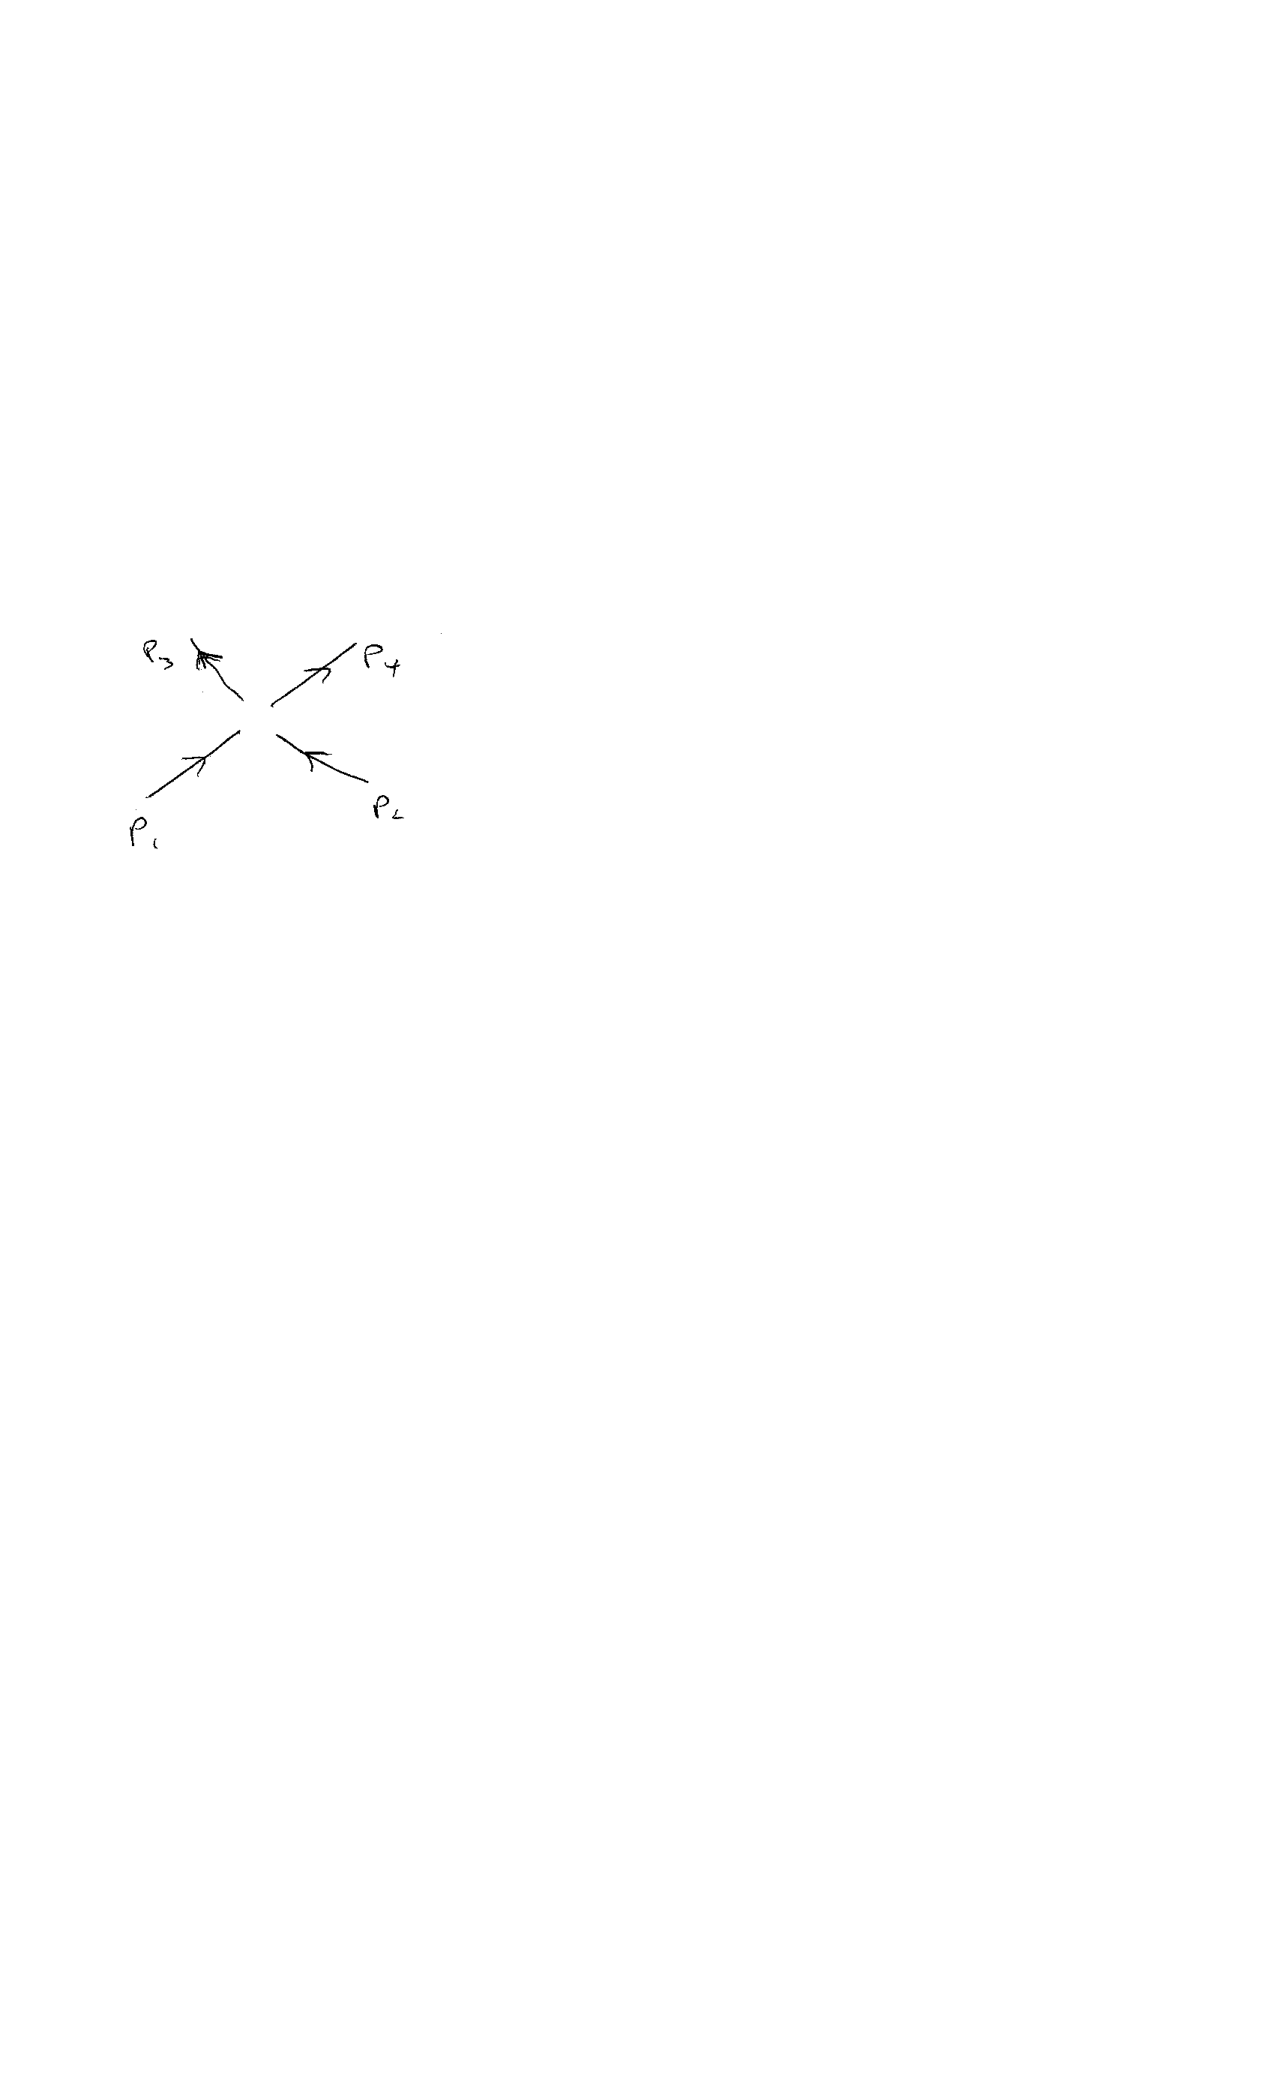
\includegraphics[width=0.4\textwidth]{./Interaction.pdf}
\end{figure}

This would correspond to adding an interaction term to the Hamiltonian of the form:

\bea
& \int \cancel{d}^3p_1 \cancel{d}^3p_2 \cancel{d}^3p_3 \cancel{d}^3p_4\ \delta(\vec{p_1}..\vec{p_4})\ \delta(E_1 + ... E_4) \\
& \underbrace{a^\dagger_{p_4,\sigma_4} a^\dagger_{p_3,\sigma_3} a_{p_2,\sigma_2} a_{p_1,\sigma_1} }_{\textrm{Acts on the initial state and gives the final state}} V(p's, \sigma's)   + \textrm{Hermitian Conjugate}
\eea

Interactions are made out of strings of a's and $a^\dagger$'s.
Also easy in this picture to talk about the creation and destruction of particles (Not just scattering) 

Very convenient to use this to map between particle states.

So far we have not said the work ``Field''. 

Now comes the challenge, 
\begin{itemize}
\item[-] These are interactions between momentum eigenstates
\item[-] Momentum Eigenstates are like big plane waves
\end{itemize}

A totally generic coefficient eg: ($\delta(\vec{p_1}..\vec{p_4}) \delta(E_1 + ... E_4) V(p's, \sigma's)$) is not going to correspond to point-like local interactions.

We would like to come up with some engine to allow us to build interaction Hamiltonians where we can just see explicitly that the interactions are local. 
This is where the utility of the field concept comes in. 


The states that we have defined act nicely under the translations operator (just pick up a phase) but to get interactions local in space we need x to make an appearance. 
That is, we want to build operators out of things like $\phi(\vec{x})$, where under T:$\phi(\vec{x}) \rightarrow \phi(\vec{x}+\vec{a})$


There is a very nice way of doing this called Fourier Transforms. 

\underline{Define}   

\be
\phi_+ (\vec{x}) = \int \cancel{d}^3p\ a^{\dagger}_{\vec{p}}\ e^{i \vec{p} \vec{x}}
\ee

and

\be
\phi_- (\vec{x}) = \int \cancel{d}^3p\ a_{\vec{p}}\ e^{-i \vec{p} \vec{x}}
\ee

Note: $\phi_- (\vec{x}) = \phi^\dagger_+ (\vec{x})$

Indeed the $\phi$'s behave as above under translations.

\noindent\rule{\textwidth}{1pt}

Can now go back to the free Hamiltonian and write it very simply using the $\phi$'s.


$\textrm{H}^{\textrm{free}}$ (non-relativistic for the moment) $E_p = p^2/2m$

\be
\textrm{H}^{\textrm{free}} = \int d^3x\ \frac{(\vec{\nabla} \phi_+ )^\dagger (\vec{\nabla} \phi_+ )}{2m}
\ee
n
which is the same as 

\be
H = \sum\limits_{p,\sigma} E_p\ a^\dagger_{p,\sigma} a_{p,\sigma}
\ee


Now its clear how you could write down interactions that take place locally:

\be
\textrm{H}^{\textrm{free}} + \int d^3x\ C[\phi_+(x)\phi_+(x)\phi_-(x)\phi_-(x)] + ... 
\ee

Its totally clear now that this is local is space. 

Taking this an expanding out gives something like we just talked about with 2a's and 2 $a^\dagger$'s.
All the rest comes along for the ride. 

(Note that this is all done non-relativistically for the moment to stress that this has nothing to do w/relativity.
This is about making interactions local)

Why we use fields: Makes local interactions of \underline{particles} manifest.

Locality is hardwired into the descriptions of particles.

So, where does relativity come in?  Where is the difficulty ?

\underline{Time Evolution}

\begin{figure}[h]
\centering
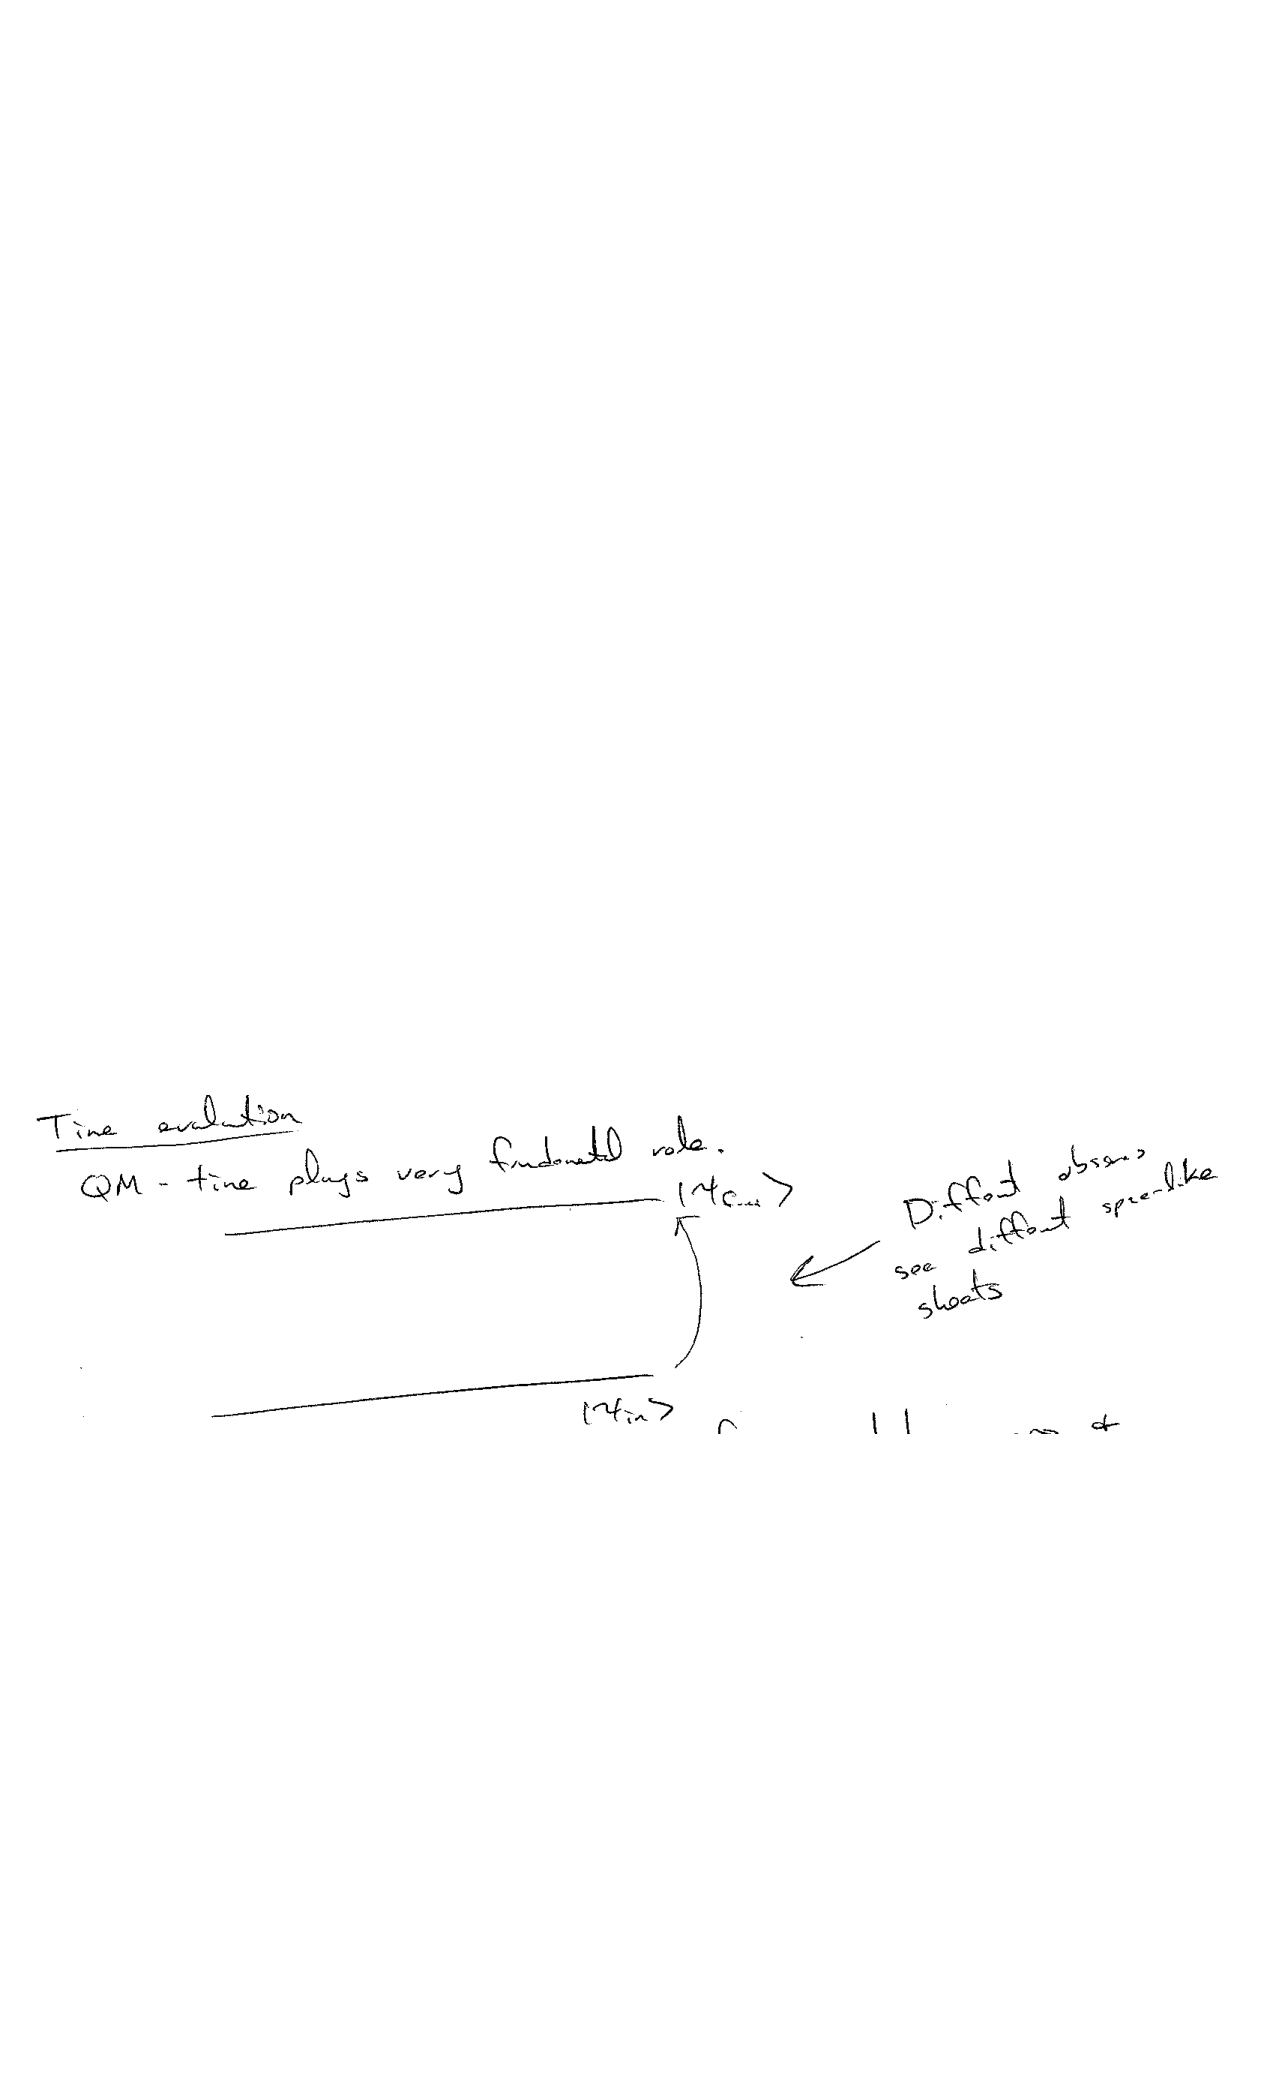
\includegraphics[width=0.9\textwidth]{./TimeEvolution.pdf}
\end{figure}

Only have a hope of Lorentz invariance if we start at -$\infty$ and go to +$\infty$.

Throw particles in from $\infty$ let them scatter \& go back out to $\infty$.

\underline{Define S-Matrix}

\be
\underbrace{\ket{p_1 \sigma_1,...p_n\sigma_n}}_{t=-\infty} \rightarrow \underbrace{\mathcal{S} \ket{p_1\sigma_1,...p_n\sigma_n}}_{t=+\infty}
\ee

}
\end{document}


